% Diese Zeile bitte -nicht- aendern.
\documentclass[course=erap]{aspdoc}
\usepackage{graphicx}
\usepackage{subcaption}
\usepackage{hyperref}
\usepackage{makecell}
\usepackage{booktabs}
\usepackage{xcolor}
\usepackage{longtable}
\usepackage{pgfplots}
\pgfplotsset{compat=1.16}
\usepgfplotslibrary{statistics}
\usepackage{tikz}
\usepackage{subcaption}

\newcommand{\theGroup}{109}
\newcommand{\theNumber}{A502}
\author{Liming Kuang \and Yaxuan Chen \and Feng Hu}
\date{Wintersemester 2021/22}

\title{Gruppe \theGroup{} -- Abgabe zu Aufgabe \theNumber}

\begin{document}
\maketitle

\section{Einleitung}
Kryptographie spielt heutzutage eine wichtige Rolle im Umfeld der Informationssicherheit. Die schafft eine Grundlage für sichere Kommunikation im Internet. Mithilfe kryptographischer Verfahren wie Verschlüsselung sollen Daten vor unbefugtem Zugriff geschützt und sicher ausgetauscht werden. Der $TEA$ \footnote{$\textbf{T}iny\ \textbf{E}ncryption\ \textbf{A}lgorithm$} \cite{10.1007/3-540-60590-8_29} ist eine der schnellsten und effizientesten kryptographischen Algorithmen, welcher die Feistelchiffre darstellt, die bekannt für ihre einfache Beschreibung und Implementierung ist. Allerdings hat der $TEA$ auch einige Schwächen, die bei den Anwendungen von den Schlüssel-Attacken ausgenutzt werden können. Um diese Schwäche zu überwinden wurden bereits viele Verbesserungsvarianten basierend auf den $TEA$ entwickelt. Der $XTEA$ \footnote{e\textbf{X}tended $\textbf{T}iny\ \textbf{E}ncryption\ \textbf{A}lgorithm$} ist eine von diesen. In den folgenden Abschnitten wird beschrieben, wie der $XTEA$ im vorliegenden Projekt in der C Sprache implementiert wurde. Dabei soll auch versucht werden, die Hauptimplementierung zu optimieren. Nach der Implementierung muss die Korrektheit der Implementierung auch noch überprüft werden. Dabei soll das Programm mit verschiedenen Eingaben und Konfigurationen getestet und die Korrektheit geprüft werden. Zu guter Letzt soll die Performanz der unterschiedlichen Implementierungen bei steigernden Größen der Eingaben analysiert und derer Performanzergebnisse dargestellt werden.

\section{Lösungsansatz}
Wie der $TEA$ ist der $XTEA$ auch eine Blockchiffre, die auf einem Feistel-Netzwerk basiert. Zuerst stellt sich die Frage, wie der Aufbau einer Feistelchiffre aussieht.

\subsection{Aufbau einer Feistelchiffre}
Unter der Feistelchiffre versteht man als eine Blockverschlüsselung, die in den 1970er Jahren von Horst Feistel \cite{feistel:1973} erfunden wurde. Diese ist eine allgemeine Struktur, mit der Blockverschlüsselungen realisiert werden können. Im Kontext der Feistelchiffre wird der Klartext in Blöcke zerlegt, die jeweils für sich verschlüsselt werden. Die Größe der Blöcke hängt vom jeweiligen Verschlüsselungsverfahren ab, oft ist sie ein Vielfaches von 64 Bits. Ein Block wird zuerst in zwei (meist gleich große) Teile geteilt: $P=L_1||R_1$, und in $n$ aufeinanderfolgenden Runden verarbeitet. In jeder Runde wird einer dieser Teile mit der Ausgabe einer Rundenfunktion verknüpft. Die Rundenfunktion erhält den anderen Teilblock und einen Rundenschlüssel als Eingabe. Innerhalb der $i$-ten Runde ($i$ läuft von 1 bis $n$) wird folgende Formel verwendet:
\begin{align*}
L_{i+1} &= R_i\\
R_{i+1} &= L_i\oplus F(R_i,\,K_i)
\end{align*}
Dabei bildet $F$ die sog. Runden- oder Transformationsfunktion und $K_1$ bis $K_n$ sind die Rundenschlüssel. $\oplus$ steht für eine einfach umkehrbare Verknüpfung. Der verschlüsselte Text am Ende der Runden ist die Zusammenführung $C=L_{n+1}||R_{n+1}$.

\subsection{Padding auf Blocklänge}
Aufgrund der Blockverschlüsselung muss die Länge der zu verschlüsselnden Daten immer ein Vielfaches der Blocklänge sein, nämlich 64-Bit. Wenn die Länge der zu verschlüsselnden Daten aber kein Vielfaches der Blocklänge ist, muss der originale Datenbestand vergrößert werden. Dieses Verfahren wird $Padding$ genannt, wobei die zur Vergrößerung der originalen Datenlänge verwendeten Bytes auch $Padding$-Bytes genannt werden.

Ein Vielfahren, das beim Padding verwendet werden kann, ist $PKCS\#7$. Dabei müssen folgende Ansprüche gestellt:

\begin{itemize}
    \item $Padding$-Bytes müssen immer vor der Verschlüsselung zum Klartext hinzugefügt werden.
    \item Jedes Auffüllungsbyte hat einen Wert, der gleich der Gesamtzahl der hinzugefügten Bytes. Wenn zum Beispiel 6 Auffüllungsbytes hinzugefügt werden müssen, hat jedes dieser Bytes den Wert von 0x6.
    \item Die mindeste Zahl der Auffüllungsbytes ist eins. Auch wenn die Länge des Klartextes bereits ein Vielfaches der Blocklänge ist, müssen in diesem Fall auch 8 Auffüllungsbytes hinzugefügt werden.
\end{itemize}

Nach dem $Padding$ kann gesichert werden, dass die Länge der zu verschlüsselnden Daten ein Vielfaches der Blocklänge ist. Jeder einzelne Block kann mit dem oben genannten $XTEA$-Verfahren verschlüsselt werden.

\subsection{Verarbeitung mehrerer Blöcke}
Um die Daten, derer Länge mehr als einem Block entspricht, mit dem Blockverschlüsselungsverfahren zu ver- bzw. entschlüsseln, muss dieses Verfahren Block für Block ausgeführt werden. Dazu gibt es verschiedene Betriebsarten, z.\,B. Electronic Code Book Mode (ECB) und Cipher Block Chaining Mode (CBC), die beschreiben, wie die Einzelblock-Operation einer Chiffre wiederholt angewendet werden kann, um Datenmengen, die größer als ein Block sind, sicher zu verschlüsseln.

Im ECB ist jeder Datenblock unabhängig von den anderen zu verschlüsseln. Dadurch ergibt, bei gleichem Schlüssel, gleicher Klartextblock immer den gleichen Geheimtextblock. Dies ist auch der größte Nachteil dieses Verfahrens, denn dadurch bleiben Klartextmuster erhalten.

Im Gegensatz zum ECB sind im CBC die Datenblöcke miteinander verkettet. Jeder Block wird nicht nur für sich allein verschlüsselt, sondern fließt der Geheimtextblock in den nächsten ein. Somit ist der Verschlüsselung eines Blocks mit dem Verschlüsselungsergebnis des vorherigen Blocks verknüpft. Das bedeutet, dass wenn sich ein Zeichen im Klartext ändert, sich (ab dem nächsten Block) auch alle weiteren Zeichen im Chiffrat ändern, auch wenn dort wieder dieselben Zeichen stehen würden. Um die Geheimtextblöcke eindeutig zu machen, auch wenn dieselben Klartexte mehrmals mit demselben Schlüssel wiederholt zu verschlüsseln sind, wird ein Initialisierungsvektor (IV) beim ersten Block verwendet.

\subsection{Kodierung in Base16}
In diesem Projekt werden die Daten in der Eingabedatei immer als $char$ eingelesen werden, welches einer Länge von 8-Bit entspricht. Diese $char$s werden mit Verschlüsselungsverfahren von $XTEA$ wieder in 8-Bit $char$s kodiert. Es kann vorkommen, dass ein $char$ zu einem $Null$-Zeichen kodiert wird und somit wird die Ausgabe der Zeichenfolge problematisch, da dieses $Null$-Zeichen als Terminal-Zeichen der Zeichenfolge erkannt wird. Außerdem, da ein zu ver- und entschlüsselnde Datenblock bei dem $XTEA$ in diesem Projekt immer 8-Byte lang ist, kann es vorkommen, dass in der Ausgabedatei nach der Verschlüsselung nicht druckbare bzw. lesbare ASCII-Zeichen enthalten sind. Um diese zu vermeiden und das Debugging zu erleichtern, werden die verschlüsselten Datenblöcke in Base16 umgewandelt. Es ist aber auch möglich, mit anderen Basen zu arbeiten, die z.\,B. in einem Internet standards track protocol \cite{RFC4648} spezifiziert sind. 

In diesem Projekt wurde aber nicht vorgeben, in welcher Basis die Daten verarbeitet werden sollen. Um einfach zu gehen, wurde die Base16 gewählt und in diesem Projekt generell verwendet.

Zur Kodierung mit Base16 werden 16 ASCII-Zeichen $A-F$ und $0-9$ verwendet. Der originale 8-Bit Datenblock wird genau in zwei Teilen von jeweils 4-Bit (entspricht einer Hex-Länge) aufgeteilt.

\subsection{Optimierung bei der Implementierung}
Der erste mögliche Optimierungsweg ist, mit SIMD 128-Bit (zweimal 64-Bit Blöcke) zu ver-/entschlüsseln. Aber nach Überlegungen stellt sich heraus, dass der aus den 64 Runden Schleifen bestehende normale $XTEA$ diffizil mit SIMD optimiert werden kann. Der Grund für die Inkompatibilität des SIMD liegt es daran, dass in einer Schleife die zwei Teilen v[0] und v[1] der 64-Bit zu verschlüsselnden Daten stark voneinander abhängig sind z.B. bei der Verschlüsselung: $v_0 \mathrel{+}= (((v_1<<4)\oplus(v_1>>5))+v_1)\oplus (sum+k[sum\&3])$. Eine andere Optimierungsmöglichkeit ist die Assemblerimplementierung, da der Assembler Code, der aus C nur ohne Optimierung kompiliert werden kann, ist grundsätzlich eine eins zu eins Übersetzung von C-Code. Daher ist es unvermeidlich, redundante Codes in den kompilierten Assembly Codes zu habe. Aus diesem Grund wäre es sinnvoll, Assembler Code selbst zu optimieren.

Darüber hinaus ist es möglich mit einer Lookup-Tablle zu optimieren. Die Grundidee ist, dass die bei der Ver-/Entschlüsselung regelmäßig durchgeführten Schritte, die aber unabhängig von der Dateneingabe sind, vorgerechnet und in einem ein-dimensionalen Feld gespeichert werden können, z.\,B. $sum+k[sum\&3]$, $sum+k[sum>>11]\&3$. In der Ver-/Entschlüsselungsprozess sind jeweils 5 Berechnungen in einer Runde weniger als die naive Implementierung. Die Operation der Berechnungen wird mit dem Zugriff der Lookup-Tabelle ersetzt und die Laufzeit ist voraussichtlich schneller.

\section{Korrektheit}
In diesem Abschnitt wird die Korrektheit der Codes geprüft, wobei das Programm nach dem Konzept der \textbf{Test Pyramid} \cite{fowler_2018} getestet wird. Die Test Pyramid zeigt, wie man verschiedene Stufen von automatisierten Tests verwenden kann, um eine robuste Testsuite zu entwickeln. Von oben nach unten besteht die originale Test Pyramid aus 3 Schichten:

\begin{itemize}
    \item End-to-End Tests (alias User Interface Tests)
    \item Service Tests
    \item Unit Tests
\end{itemize}
    
Da das Projekt relativ klein und unkompliziert ist, wird eine vereinfachte Version dieses Modells verwendet, die ausschließlich aus \textit{End-to-End Tests} und \textit{Unit Tests} besteht. \textit{End-to-End Tests} sind hoch integrierte Tests, die das tatsächliche Benutzerverhalten in einem realen Szenario imitieren. Daher haben wir ein einfaches Bash-Shell-Skript geschrieben, das automatisch eine Reihe von Befehlen ausführt, nicht nur die, die vom Programm unterstützt, sondern auch die vom Programm nicht unterstützt sind. Auf diese Weise kann die allgemeine Korrektheit unseres Programms relativ effizient überprüft werden. \textit{Unit Tests} sind eher isolierte Tests, mit denen die Korrektheit jeder einzelner Funktionsimplementierung verifiziert werden kann. Aufgrund der großen Anzahl der Funktionen des Programms werden einige der wichtigsten Funktionen für Unit Test herausgepickt. Hier werden die allgemeinen Korrektheit aller Funktionen getestet, und zusätzlich gibt es spezifische Tests für Sonder-/Randfälle.

\subsection{Exemplarische Programmausgabe}
Es wird in Tabelle \ref{tab:io} gezeigt, wie eine typische Ausgabe des Programms mit verschiedenen Eingaben aussehen würde(> ist der Bash Prompt Indikator):

\begin{table}[ht]
    \centering
    \footnotesize
    \begin{tabular}{p{0.06\linewidth}p{0.51\linewidth}p{0.33\linewidth}}
    \toprule[2pt]
    \textbf{Input}  &  > ./main ./test/input.txt & \textcolor{magenta}{\% einfachste mögliche Eingabe} \\
    \specialrule{0.1pt}{2pt}{2pt}
    \textbf{Output}   &  \makecell[l]{ENCRYPT SUCCESS \\ EVERYTHING OK} & \\
    \midrule
    
    \textbf{Input}  &  \makecell[l]{> ./main -V0 -B100 ./test/input.txt -k 1,2,3,4 -i 5,6 \\-o ./test/output.txt} & \makecell[l]{\textcolor{magenta}{\% eine vollständige Eingabe mit} \\ \textcolor{magenta}{Benchmark}} \\
    \specialrule{0.1pt}{2pt}{2pt}
    \textbf{Output}   &  \makecell[l]{Total runtime for running 100 times: 0 seconds and 4067555 nanoseconds\\
    Average runtime for running 100 times: 0 seconds and 40675 nanoseconds\\
    Total time for 100 times encryption/decryption: 0 seconds and 93575 nanoseconds\\
    Average time for 100 times encryption/decryption: 0 seconds and 935 nanoseconds\\
    EVERYTHING OK} & \\
    \midrule
    
    \textbf{Input}  &  > ./main & \textcolor{magenta}{\% eine Eingabe ohne Eingabedatei} \\
    \specialrule{0.1pt}{2pt}{2pt}
    \textbf{Output}   &  \makecell[l]{Error: No input file specified} & \\
    \bottomrule[2pt]
    \end{tabular}
    \caption{Normaler Input/Output}
    \label{tab:io}
\end{table}

Das erste Beispiel ist eine Eingabe, die kein Benchmarking erfordert. Es würde zunächst die Nachricht ''\textbf{ENCRYPT SUCCESS}'' anzeigen, die den Erfolg des Ver-/Entschlüsselungsprozesses bestätigt. Danach folgt ein ''\textbf{EVERYTHING OK}'', welches anzeigt, dass das Ergebnis erfolgreich in die entsprechende Ausgabedatei geschrieben wurde. Für ein Benchmarking würden zuerst die Gesamt- und Durchschnittslaufzeit des gesamten Programms und dann die Gesamt- und Durchschnittslaufzeit für den Ver-/Entschlüsselungsprozess allein ausgegeben werden (beide in Nanosekunden für mehr Genauigkeit). Dann folgt ein ''\textbf{EVERYTHING OK}'' ganz am Ende, um anzuzeigen, dass das Ergebnis in die Ausgabedatei geschrieben wurde. Schließlich wird demonstriert, wie es mit einer Fehlermeldung umgeht. Die beginnt mit einem ''\textbf{Fehler: } '', gefolgt von einer ausführlichen Erläuterung des aufgetretenen Fehlers, die dem Benutzer helfen soll, herauszufinden, wo und wie er/sie den Fehler beheben kann. 

\subsection{End-to-End Test}
Für den End-to-End Test wurde ein Bash-Skript \lstinline{e2etest.sh} und eine Eingabedatei \lstinline{e2e_in.txt} geschrieben, die im Pfad \lstinline{./Implementation/test/} zu finden ist. Als Voraussetzung der Ausführung des Skripts in $lxhalle$, müssen zuerst \lstinline{chmod u+x ./e2etest.sh} und dann das Skript mit \lstinline{bash ./e2etest.sh} ausgeführt werden. In dem Skript sollen vier der häufigsten Anwendungsfälle des Programms getestet werden, nämlich schnelle Ver-/Entschlüsselung mit nur einer Eingabedatei und Ver-/Entschlüsselungsbenchmarking mit einer alternativen Implementierung für 20 Runden mit einem angegebenen Schlüssel, einem Initialisierungsvektor und einem Ausgabedateinamen. Dann wird die Ausgabe des Programms mit Regex geparst, um zu bestimmen, ob die Ausgabemeldung korrekt ist, die Ausgabedatei mit dem richtigen Dateinamen existiert und der Inhalt der Ausgabedatei korrekt ist. 
Dann sind insgesamt 11 verschiedene möglichen ungültigen Eingaben aufgelistet. Es wird getestet, ob das Programm den Fehler korrekt abfangen und eine relevante und sinnvolle Fehlermeldung für den Benutzer ausgeben kann. Dazu gehören Fehler wie:
\begin{itemize}
    \item Existiert die Eingabedatei? Gibt es mehrere Eingabedateien?
    \item Ist das Format von Schlüssel/IV korrekt? Ergibt der Schlüssel/IV-Wert Sinn (z. B.: nicht-ganzzahlige Zeichen)?
    \item Ist der Schlüssel für die Entschlüsselung falsch?
    \item Ist die Rheinfolge der Optionen richtig?
    \item Ist die Option bekannt? Sind die Argumente für eine bestimmte Option gültig?
\end{itemize}
Im Bash-Skript ist eine vollständige Liste der getesteten ungültigen Eingaben zu finden. Tabelle \ref{tab:e2e} zeigt einen Ausschnitt davon, wie das Skript läuft und wie das Programm sich verhält.

{\centering
\footnotesize    
\begin{longtable}{p{0.06\linewidth}p{0.85\linewidth}}
    
    \toprule[2pt]
    \textbf{Input}  &  > ./e2etest.sh  \\
    \midrule
    
    \textbf{Output}   &  \makecell[l]{
    Welcome to the E2E Test Script of Project Team 109 -- XTEA En/Decryption\\
    Input file: e2e\_in.txt\\
    ...\\
    Test 1: The most simple encrypt command possible:\\
    Command: ../main e2e\_in.txt\\
    ENCRYPT SUCCESS\\
    EVERYTHING OK\\
    Test 1 PASS\\
    ...\\
    Test 5: Error handling for invalid inputs:\\
    No input file: PASS\\
    Multiple input file: PASS\\
    Wrong args sequence: PASS\\
    ...\\
    Total error handled: 10 / 10\\
    Test 5 PASS} \\

    \bottomrule[2pt] 
    \caption{End-to-End Test Ergebnis}
    \label{tab:e2e}\\
\end{longtable}}


\subsection{Unit Test}


Für den Unit Test ist die Datei \lstinline{unittest.c} im Ordner \lstinline{./Implementation} zu finden. Zuerst soll die Datei mit dem Befehl \lstinline{make unittest} kompiliert und dann mit dem Befehl \lstinline{./unittest} ausgeführt werden.


In diesem Unit Test werden 9 wichtigsten C-Funktionen des Programms getestet. Sie sind in Tabelle \ref{tab:ut_funcs} zu finden.


\begin{table}[h]
    \centering
    \footnotesize 
    \begin{tabular}{p{0.23\linewidth}p{0.72\linewidth}}
    \toprule[2pt]
        Funktion Name & Beschreibung\\
        \midrule
         args\_parser &  Alle Argumenten der Eingabebefehl parsen \\
         read\_file & Datei einlesen und mögliche Fehler erkennen\\
         write\_file & Daten in eine Datei schreiben und mögliche Fehler erkennen\\
         xtea\_encrypt\_block & Ein Textblock verschlüsseln\\
         xtea\_decrypt\_block & Ein Block von Chiffre verschlüsseln\\
         binary\_to\_hex & Ein binäres char* in ein hexadezimales char* konvertieren\\
         hex\_to\_binary & Ein hexadezimales char* in ein binäres char* konvertieren\\
         xtea\_encrypt & Eingabe padden und dann verschlüsseln\\
         xtea\_decrypt & Die Chiffre entschlüsseln\\
    \bottomrule[2pt]
    \end{tabular}
    \caption{List aller von Unit Test getesteten Funktionen}
    \label{tab:ut_funcs}
\end{table}


Die grundlegende Logik hinter den Unit Tests ist, dass jede Funktion mit einer bestimmten Eingabe auszuführen ist, die eine bekannte erwartete Ausgabe hat. Dann wird das von der Funktion gelieferte Ergebnis mit dem erwarteten Ergebnis mithilfe einer C-Funktion \lstinline{void assert(scalar expression)} aus der Library \lstinline{"assert.h"} verglichen. Wenn beide Ergebnisse gleich sind, läuft der Unit Test weiter. Wenn nicht, bricht es mit einer Fehlermeldung ab, die angibt, wo der Fehler liegt. Mit dieser Methode werden und allgemeine Fälle einzelner Funktionen und Randfalle automatisch und effizient getestet. Der allgemeine Fall aller oben genannten Funktionen wurde getestet und in Tabelle \ref{tab:ut_edgecase} sind noch einige Randfälle, die getestet wurden, aufgelistet. Da C keine native try/catch-Unterstützung bietet, werden einige Randfälle, z.\,B.: Implementierungsnummern, die außerhalb des zulässigen Bereichs liegen, im End-to-End Test mit einem Bash-Skript getestet. Eine umfassende Liste von allen 22 Unit Tests sind im Code zu finden. 


\begin{table}[h]
    \centering
    \footnotesize 
    \begin{tabular}{p{0.2\linewidth}p{0.75\linewidth}}
    \toprule[2pt]
         Funktion Name & Getestete Randfälle\\
        \midrule
         xtea\_encrypt\_block & Maximale/Minimale zu-verschlüsselte Daten\\
         xtea\_decrypt\_block & Maximale/Minimale zu-entschlüsselte Daten\\
         binary\_to\_hex & 0xFFFFFFFF/0x00000000 als Eingabe \\
         hex\_to\_binary & ''FFFFFFFF''/''00000000'' als Eingabe\\
         xtea\_encrypt & Wenn Länge der Text < oder == Blocklänge\\
         xtea\_decrypt & Wenn Länge der originale Text < oder == Blocklänge\\
    \bottomrule[2pt]
    \end{tabular}
    \caption{List der Randfälle}
    \label{tab:ut_edgecase}
\end{table}

Tabelle \ref{tab:ut_res} zeigt einen Auszug aus der Ausgabe der Unit Tests:

{\centering
\footnotesize    
\begin{longtable}[h]{p{0.06\linewidth}p{0.85\linewidth}}
    
    \toprule[2pt]
    \textbf{Input}  &  > ./unittest  \\
    \midrule
    
    \textbf{Output}   &  \makecell[l]{
    Welcome to the Unit Test of Project Team 109 -- XTEA En/Decryption\\
    The unit test will test the following functions:\\
    ...\\
    Argument parsing correct\\
    File reading correct\\
    ...\\
    All tests passed!} \\

    \bottomrule[2pt] 
    \caption{Ergebnis der Unit Tests}
    \label{tab:ut_res}\\
\end{longtable}}



\section{Performanzanalyse}
Im Folgenden werden die Ergebnisse der Performanzanalyse des Programms präsentiert. Die Performanzanalyse besteht aus der Laufzeitanalyse des Programms mit dem Profiling Tool und dem Vergleich zu anderen optimierten Implementierungen. \vspace{80mm}
Im ersten Schritt wird die Laufzeit des ganzen Programms mithilfe Profiling Tool analysiert. Außerdem wird der Zeitaufwand anhand eines Beispiels analysiert und bewertet. Im zweiten Schritt geht es darum, das Vergleichsergebnis grafisch darzustellen und zu bewerten.

\subsection{Laufzeitanalyse des Programms}
In den folgenden Abschnitten wird das gewählte Profiling Tool erklärt. Zudem werden alle Faktoren, die die Laufzeit beeinflussen können, anhand eines Beispiels diskutiert und bewertet.

\subsubsection{Profiling Methode}
Als Profiling-Tool wurde der GNU Profiler \cite{gnu_profilier} entschieden, der am 1993 von Jeffrey Osier veröffentlicht und am 1997 von Brent Baccala erneuert wurde. Der im Vorlesungsvideo vorgestellte Befehl \textbf{-perf}  funktioniert nicht wirksam, da die Funktionsnamen jeder Funktion nicht sichtbar sind. 
Aus diesem Grund wird der GNU Profiler verwendet, um den Anteil der Laufzeit jeder Funktionen zu protokollieren. Vor dem Profiling muss das Programm mit dem Flag \textbf{-pg} kompiliert und danach muss der folgende Befehl ausgeführt werden:

\begin{center}
        \textbf{\textit{-gprof options [executable-file [profile-data-files...]] [> outfile] |less}} 
\end{center}

Nach jeder Ausführung werden alle wissenswerten Daten über den Zeitaufwand des Programmes tabellarisch dargestellt.

\subsubsection{Profilingsergebnis Beispiel}
Aus den zahlreichen Werten des Profilingsergebnisses werden nur zwei davon betrachtet: erstens der Anteil der Zeitverteilung des Programms in Potenz, zweitens die Namen der aufgerufenen Funktionen. Im Gegensatz zur Protokollierung der Zeitverteilung in Potenz ist die sekündliche Laufzeit sinnlos, da die proportional zur Wiederholungsanzahl ist.

\begin{table}[h]
    \centering
    \footnotesize 
    \begin{tabular}{p{0.1\linewidth}p{0.2\linewidth}}
    \toprule[2pt]
         Zeit in \% & Funktion Name\\
        \midrule
         90.20 & xtea\_encrypt\_block\\
         8.78 & binary\_to\_hex\\
         0.00 & parse\_string\_to\_array\\
         0.00 & read\_file\\
    \bottomrule[2pt]
    \end{tabular}
    \caption{Profilingsergebnis}
    \label{tab:profiling_ergebnis}
\end{table}

Um die Laufzeit des Programmes besser zu erläutern, wird ein Profilingsergebnis als ein Beispiel herangezogen. In Tabelle \ref{tab:profiling_ergebnis} wird das Teilergebnis eingetragen, das mit der Operation \textit{./main -B2000 -V0 test/1000k.txt -k 2,3,4,5 -i 13,25 -o test/output.txt} erzeugt wurde. Getestet wurde auf einem System mit einem AMD Ryzen 5 3600 6-Core Prozessor, 3.60 GHz, 16 GB Arbeitsspeicher, Ubuntu 20.04.3, Linux-Kernel 5.4.0. Kompiliert wurde mit GCC Version 9.4.0 mit der Optimierungsoption -O2.

\subsubsection{Profilingsbewertung}
In Tabelle \ref{tab:profiling_ergebnis} wird es verdeutlicht, dass der Zeitaufwand hauptsächlich aus zwei Teilen besteht: Verschlüsselung $xtea\_encrypt\_block$ und Hex-codierung $binary\_to\_hex$.

Laut Ergebnis des Zeitaufwandes beträgt die Laufzeit der Verschlüsselungsfunktion $xtea\_encrypt\_block$ 90.20\,\% der Gesamtlaufzeit, welches der Implementierung entspricht, bei der jeder Datenblock 64 Runden wiederholt berechnet wird. Das gewählte Ver-/Entschlüsselungsverfahren ist $XTEA$ mit der Betriebsart von CBC. Anders als EBC wird bei CBC eine $XOR$-Operation vor und nach normaler Ver-/Entschlüsselung mit dem Initialisierungsvektor durchgeführt. Es ist fraglos, dass mit CBC die Sicherheit der Ver-/Entschlüsslung besser garantiert werden kann, aber hingegen der Zeitaufwand erhöht wird.

Außerdem muss der Hexencodierungsprozess, der 8.78\,\% der Gesamtlaufzeit verbraucht, nur einmal für den ganzen zu verschlüsselnden Daten durchgeführt. Die Hex-codierung (Base16) spielt eine Rolle, um die mit $XTEA$ verschlüsselten Geheimtexte in Hexadezimal-Form darzustellen. Für jedes Zeichnen wird die Hex-codierung einmal durchgeführt. Somit wird die Geheimtextlänge doppelt so groß.

\subsection{Zeitmessungsmethodik}
Die Zeitmessung ist im Benchmark File mithilfe der Funktion \lstinline{clock_gettime(CLOCK_MO-NOTONIC, struct timespec *res)} berechnet. Vor und nach der Ver-/Entschlüsselung wird die verbrauchte Zeit in Nanosekunden gemessen und aufsummiert. Falls die gemessene Zeit mehr als eine Sekunde ist, wird die Zeit abgerundet. Am Ende wird die Summe der Zeit durch Wiederholungsanzahl geteilt und enthält die durchschnittliche Laufzeit. Alle Tests sind in einer kontinuierlichen Zeit durchgeführt, um die Abweichungen am möglichsten zu verringern.

\subsection{Naive C Implementierung vs. Assemblerimplementierung}
Die Assemblerimplementierung ist eine andere Version, mit der die native C Implementierung zu vergleichen ist. Im Programm wurden die Ver-/Entschlüsselungsverfahren der C Implementierung in Assembly Sprache umgeschrieben. Getestet wurde auf einem System mit einem AMD Ryzen 5 3600 6-Core Prozessor, 3.60GHz, 16 GB Arbeitsspeicher, Ubuntu 20.04.3, Linux-Kernel 5.4.0. Kompiliert wurden mit GCC Version 9.4.0 mit der Optimierungsoptionen -O2. Die benutzten Schlüssel waren in Form 2,3,4,5 und der Initialisierungsvektor war in Form 13,57.

Die Berechnungen der Laufzeit wurden mit Eingabegrößen von $5*10^6$ bis $45*10^6$ Zeichnen jeweils 20-mal durchgeführt und die durchschnittliche Laufzeit der Ver-/Entschlüsslung in Millisekunden wurde für jede Eingabegröße in Abbildung \ref{fig:En/Decryption CAssembly Vergleich} dargestellt.

\begin{figure}[!ht]
\begin{subfigure}[t]{.5\textwidth}
    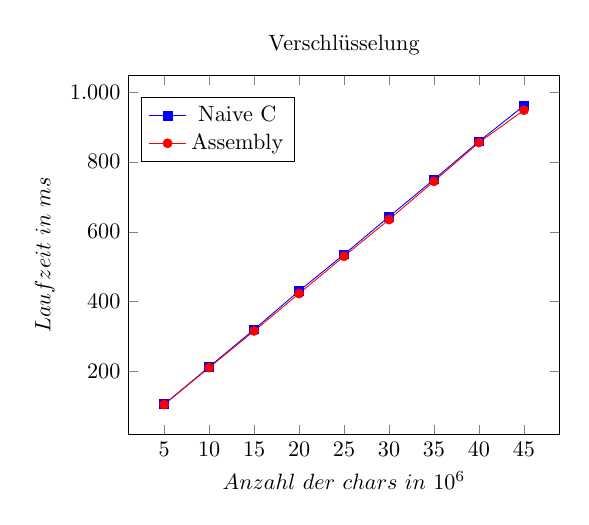
\begin{tikzpicture}[xscale=0.8, yscale=0.8]
        \begin{axis}[xlabel={$Anzahl\ der\ chars\ in\ 10^6$}, ylabel={$Laufzeit\ in\ ms$}, title=Verschlüsselung, legend style={at={(0.03,0.85)}, anchor=west}, ylabel near ticks, xtick distance={5}, y tick label style={/pgf/number format/.cd, set thousands separator={.}}]
            \addplot[blue][mark=square*] coordinates { (5,106.45) (10,213.41) (15,320.43) (20,430.69) (25,535.11) (30, 642.98) (35,749.44) (40,858.33)(45,960.41) };
            \addplot[red][mark=*] coordinates { (5,105.64) (10,211.44) (15,316.25) (20,423.17) (25,529.85) (30,634.66) (35,744.25)(40,855.11)(45,947.66) };
            \addlegendentry{Naive C}
            \addlegendentry{Assembly}
        \end{axis}
    \end{tikzpicture}
\end{subfigure}
\begin{subfigure}[t]{.5\textwidth}
    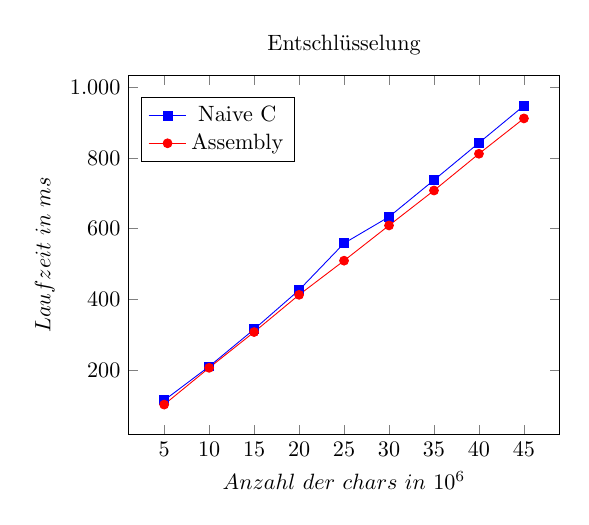
\begin{tikzpicture}[xscale=0.8, yscale=0.8]
        \begin{axis}[xlabel={$Anzahl\ der\ chars\ in\ 10^6$}, ylabel={$Laufzeit\ in\ ms$}, title=Entschlüsselung, legend style={at={(0.03,0.85)}, anchor=west}, ylabel near ticks, xtick distance={5}, y tick label style={/pgf/number format/.cd, set thousands separator={.}}]
            \addplot[blue][mark=square*] coordinates { (5,114.36) (10,209.97) (15,315.14) (20,426.18) (25,558.43) (30,633.25) (35,737.24) (40,842.49) (45,947.56) };
            \addplot[red][mark=*] coordinates { (5,102.16) (10,206.19) (15,307.36) (20,412.66) (25,509.24) (30,608.90) (35,707.75) (40,811.68) (45,911.64) };
            \addlegendentry{Naive C}
            \addlegendentry{Assembly}
        \end{axis}
    \end{tikzpicture}
\end{subfigure}
\caption{Naive C Implementierung vs. Assemblerimplementierung}
    \label{fig:En/Decryption CAssembly Vergleich}
\end{figure}

\subsection{Naive C Implementierung vs. C Implementierung mit Lookup-Tabelle}
Der Test wurde in der identischen Testumgebung wie der Test mit der Assemblerimplementierung durchgeführt. Die benutzten Schlüssel waren ebenfalls in Form 2,3,4,5 und der Initialisierungsvektor war in Form 13,57. 

\begin{figure}[!ht]
\begin{subfigure}[t]{.5\textwidth}
    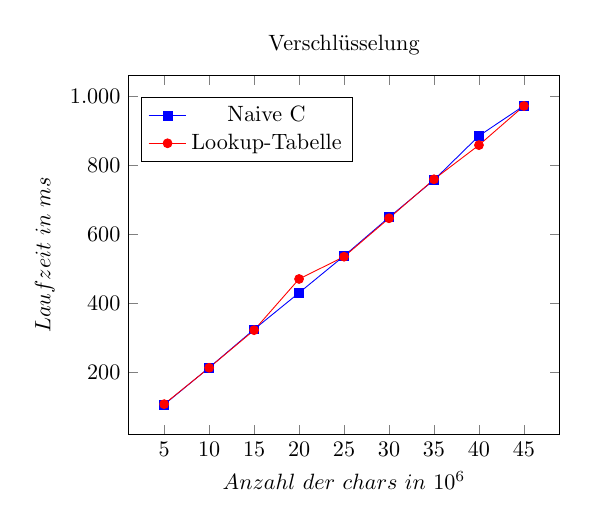
\begin{tikzpicture}[xscale=0.8, yscale=0.8]
        \begin{axis}[xlabel={$Anzahl\ der\ chars\ in\ 10^6$}, ylabel={$Laufzeit\ in\ ms$}, title=Verschlüsselung, legend style={at={(0.03,0.85)}, anchor=west}, ylabel near ticks, xtick distance={5}, y tick label style={/pgf/number format/.cd, set thousands separator={.}}]
            \addplot[blue][mark=square*] coordinates { (5,107.21) (10,214.28) (15,325.10) (20,431.00) (25,537.81) (30, 649.69) (35,757.83) (40,885.56)(45,972.88) };
            \addplot[red][mark=*] coordinates { (5,108.55) (10,213.84) (15,322.83) (20,471.07) (25,535.56) (30,646.91) (35,759.81)(40,858.79)(45,972.11) };
            \addlegendentry{Naive C}
            \addlegendentry{Lookup-Tabelle}
        \end{axis}
    \end{tikzpicture}
\end{subfigure}
\begin{subfigure}[t]{.5\textwidth}
    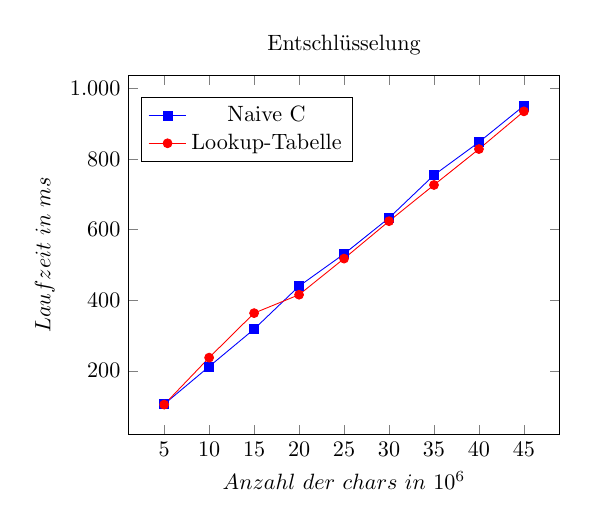
\begin{tikzpicture}[xscale=0.8, yscale=0.8]
        \begin{axis}[xlabel={$Anzahl\ der\ chars\ in\ 10^6$}, ylabel={$Laufzeit\ in\ ms$}, title=Entschlüsselung, legend style={at={(0.03,0.85)}, anchor=west}, ylabel near ticks, xtick distance={5}, y tick label style={/pgf/number format/.cd, set thousands separator={.}}]
            \addplot[blue][mark=square*] coordinates { (5,105.26) (10,212.01) (15,318.09) (20,439.99) (25,531.28) (30,633.33) (35,754.94) (40,848.28) (45,951.57) };
            \addplot[red][mark=*] coordinates { (5,104.12) (10,237.31) (15,363.50) (20,415.71) (25,518.13) (30,624.16) (35,726.86) (40,828.68) (45,935.62) };
            \addlegendentry{Naive C}
            \addlegendentry{Lookup-Tabelle}
        \end{axis}
    \end{tikzpicture}
\end{subfigure}
\caption{Naive C Implementierung vs. C Implementierung mit Lookup-Tabelle}
    \label{fig:En/Decryption Vergleich mit Lookup-Tabelle}
\end{figure}

\subsubsection{Vergleichsbewertung}
In Abbildung \ref{fig:En/Decryption CAssembly Vergleich} wird es verdeutlicht, dass die Assemblerimplementierung kaum optimiert ist. Laut der gemessenen Zeit ist die Assemblerimplementierung bei der Verschlüsselung 1.3\,\% und bei der Entschlüsselung 3.8\,\% schneller als die naive C Implementierung. Der Grund dafür ist, dass der selbstgeschriebene Assembler Code nicht deutlich effizienter als der mit -O2 Flag kompilierte Code ist. Die Anzahl der Instruktionen der vom Compiler geschriebene Assembly Codes ist ähnlich wie die selbst geschrieben Assembly Codes.

In Abbildung \ref{fig:En/Decryption Vergleich mit Lookup-Tabelle} wird es veranschaulicht, dass die Optimierung mit der Lookup-Tabelle ineffizient und in einigen Fällen die Laufzeit sogar verschlechtert. Die Implementierung mit einer Lookup-Tabelle vergrößert die Möglichkeit der Cache-Miss beim Zugriff des Feldes. Die im $XTEA$ verwendeten Operationen z.\,B. $XOR$ oder bitweise Schiebeoperationen sind effizient für CPU. Wenn es eine Cache-Miss passiert, dann wird das Programm langsamer als die mit -O2 Flag opitimierte naive C Implementierung.

\section{Zusammenfassung und Ausblick}
In diesem Projekt wurde ein Blockchiffre-Algorithmus $XTEA$ mit Ver- und Entschlüsselungsverfahren implementiert, der nach dem Konzept der Feistelchiffre auggebaut wurde. Da der Blockchiffre-Algorithmus nur die Daten mit einer vielfachen Länge der Blocklänge (64-Bit in diesem Projekt) behandeln kann, müssen die Daten, derer Länge kein Vielfaches der Blocklänge ist, mit dem sogenannten $Padding$-Verfahren mit Padding-Bytes aufgefüllt werden. Dabei wurde das $PKCS\#7$ verwendet. Wenn im originalen Datenbestand mehr als ein Block vorliegen, müssen die Datenblöcke mit den Ver- und Entschlüsselungsverfahren in Kombination von Betriebsarten verarbeitet werden. Dazu wurde in diesem Projekt der CBC angesetzt, da dieser eine sichere Betriebsart im Umfeld der Kryptographie vergleichend zu ECB ist. Um die Probleme bei der Ausgabe der ASCII-Zeichen aufgrund $Null$-Zeichen zu vermeiden und auch lesbare Zeichen in der Ausgabedatei für das Debugging zu ermöglichen, wurden in diesem Projekt die verschlüsselten Blöcke in $Base16$ umgewandelt.

Um die Korrektheit der Implementierung zu überprüfen, wurden sowohl der End-to-End Test als auch der Unit Test durchgeführt. Dabei wurden die Wirksamkeit und Korrektheit sowohl bei den Optionen, die in der Kommandozeile eingegeben werden, als auch bei den Funktionen wie z.\,B. $args\_parser$, $read\_file$, $write\_file$ mit verschiedenen Test-Fällen getestet.

Zu guter Letzt wurde die Performanz sowohl der Hauptimplementierung in C Sprache als auch die alternativen Implementierungen in der Assembly Sprache und mit einer Lookup-Tabelle analysiert. Daraus wurde aber gemerkt, dass die Hauptimplementierung bei der Kompilierung mit -O2 Flag vergleichend zu Assemblerimplementierung fast gleiches Performanzsniveau hatte. Aufgrund Cach-Miss beim Speicherzugriff mit einer Lookup-Tabelle hat diese Implementierung ebenfalls keine besssere Performanz gezeigt.

\bibliographystyle{plain}
\bibliography{Ausarbeitung}{}
\end{document}
